% !TeX spellcheck = pl_PL

\rozdzial

%%%%%%%%%%%%%%%%%%%%%%%%%%%%%%%%%%%%%%%%%%%%%%%%%%%%%%%%%%%%%%%%%%%%%%%
\section{Logowanie i zarządzanie dostępem}

\subsection{Logowanie}

Program uruchamia się za pomocą dwukrotnego kliknięcia na ikonę DotBase.exe.
Po uruchomieniu aplikacji pojawia się okno logowania (rys. \ref{oknoLogowania}).

W prawym dolnym rogu okna znajduje się aktualna wersja programu.

\begin{figure}[htb]
	\centering
	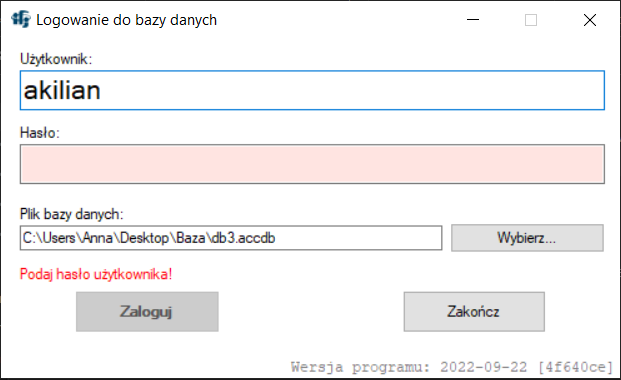
\includegraphics{obrazki/Logowanie/logowanie.png}
	\caption{Okno logowania}
	\label{oknoLogowania}
\end{figure}

W pierwszej kolejności należy podać bezwzględną ścieżkę do pliku bazy danych, na której zamierza się pracować. Można również wybrać plik bazy, korzystając z przycisku \textbf{"Wybierz..."}, który otwiera okno eksploratora plików Windows. 

\textbf{TIP:} Program zapamiętuje ostatnią podaną ścieżkę i automatycznie wpisuje ją przy kolejnym uruchomieniu.

\textbf{TIP:} Na jednym pliku bazy danych może pracować jednocześnie kilkoro użytkowników na różnych komputerach podłączonych do wspólnej sieci lokalnej.

Jeżeli ścieżka do bazy danych jest wybrana należy wpisać przydzielony login i hasło i nacisnąć przycisk \textbf{"Zaloguj"}. Program automatycznie sprawdza czy wczytana baza danych posiada wszystkie odpowiednie tabele i ustawienia wymagane do jego prawidłowej pracy.
Jeżeli mamy uprawnienia administratora, to po wpisaniu poprawnego loginu i hasła pojawia się dodatkowy przycisk \textbf{"Administracja"} (rys. \ref{oknoLogowaniaAdmina}). Przycisk ten przenosi nas do części programu związanej z zarządzaniem hasłami i dostępem użytkowników (patrz rozdz. \ref{admin}).

\begin{figure}[htb]
	\centering
	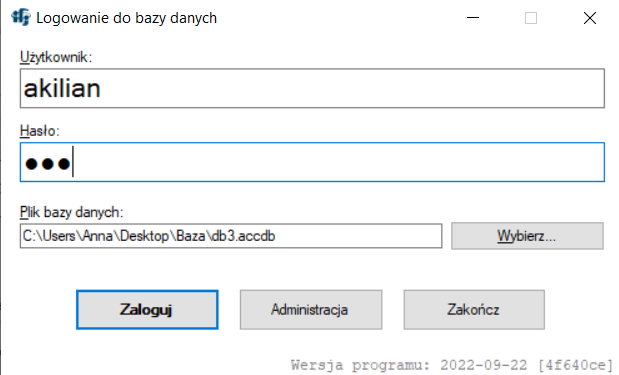
\includegraphics{obrazki/Logowanie/logowanie_administracja.png}
	\caption{Okno logowania administratora}
	\label{oknoLogowaniaAdmina}
\end{figure}

Po zalogowaniu przechodzimy bezpośrednio do menu głównego programu (rys. \ref{menuGlowne}). Stąd możemy przejść do poszczególnych modułów programu:
\begin{itemize}
	\item \textbf{"Biuro"} - wprowadzanie zleceń i przyrządów, ustalanie cen, przygotowywanie meldunków - patrz rozdz. \ref{biuro}
	\item \textbf{"Wzorcowanie"} - wprowadzanie wyników wzorcowania, obliczenia parametrów kalibracji, przygotowywanie protokołów, świadectw i pism przewodnich - patrz rozdz. \ref{wzorcowanie}
	\item \textbf{"Wyszukiwanie"} - różnego rodzaju wyszukiwania i statystyki - patrz rozdz. \ref{wyszukiwanie}
	\item \textbf{"Ustawienia"} - zmiana ustawień, parametrów, wprowadzanie danych wzorcowych - patrz rozdz. \ref{ustawienia}
\end{itemize}

Wciśnięcie przycisku \textbf{"Wyloguj"} spowoduje wylogowanie z programu i przejście ponownie do okna logowania (rys. \ref{oknoLogowania}).

\begin{figure}[htb]
	\centering
	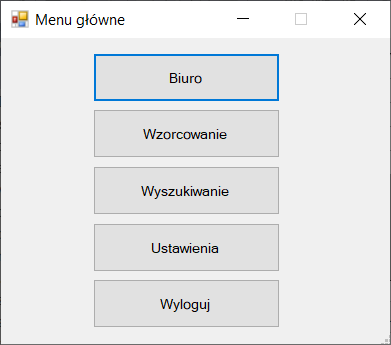
\includegraphics{obrazki/Logowanie/menu_glowne.png}
	\caption{Menu główne}
	\label{menuGlowne}
\end{figure}

\subsection{Administracja}
\label{admin}

Ta część programu pozwala zarządzać dostępem użytkowników do bazy danych (rys. \ref{administracja}). Jest tu lista wszystkich użytkowników mających uprawnienia do przeglądania i~edycji bazy danych. Można dodawać kolejnych poprzez wpisanie ich do tabeli. Usunięcie zaznaczonego użytkownika następuje po wciśnięciu przycisku \textbf{"Usuń użytkownika"}. Z tego poziomu można także nadawać lub odbierać uprawnienia administratora poprzez zaznaczenie lub odznaczenie pola wyboru w kolumnie \textbf{"Administrator"}.

\begin{figure}[htb]
	\centering
	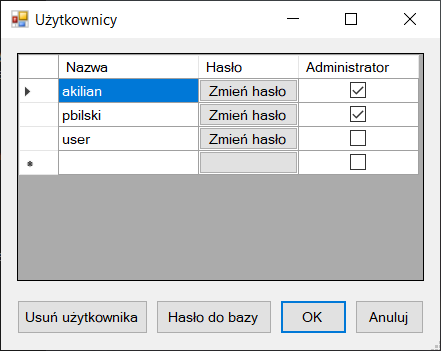
\includegraphics{obrazki/Logowanie/administracja.png}
	\caption{Okno zarządzania dostępem użytkowników}
	\label{administracja}
\end{figure}

Po wciśnięciu przycisku \textbf{"Hasło do bazy"} otwiera się kolejne okno umożliwiające zmianę ogólnego hasła do bazy danych (pliku MS Access). Hasło powinno być nie krótsze niż 8 znaków i zawierać co najmniej jedną literę i jedną cyfrę. Zmianę hasła należy zatwierdzić wciskając przycisk \textbf{"OK"}.

\textbf{Ważne:} Aby zmienić ogólne hasło do bazy danych należy znać aktualne hasło.

\begin{figure}[htb]
	\centering
	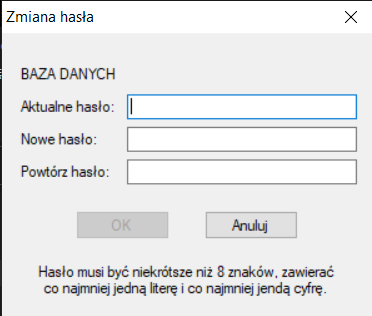
\includegraphics{obrazki/Logowanie/zmiana_hasla_bazy.png}
	\caption{Okno zmiany hasła do bazy danych}
	\label{zmianaHaslaBazy}
\end{figure}

Aby zmienić hasło logowania do programu dla danego użytkownika należy wcisnąć odpowiadający mu przycisk "Zmień hasło" (kolumna "Hasło"). Hasło powinno być nie krótsze niż 8 znaków i zawierać co najmniej jedną literę i jedną cyfrę. Zmianę hasła należy zatwierdzić wciskając przycisk \textbf{"OK"}.

\textbf{TIP:} Aby zmienić hasło użytkownika nie trzeba znać jego aktualnego hasła. Jest to więc funkcja przydatna do zresetowania hasła w przypadku, kiedy użytkownik zapomni swojego hasła.

Użytkownik może sam zmienić swoje hasło. Jest to opcja dostępna w menu \textbf{"Ustawienia"} - patrz rozdz. \ref{zmiana_hasla}. 

\begin{figure}[H]
	\centering
	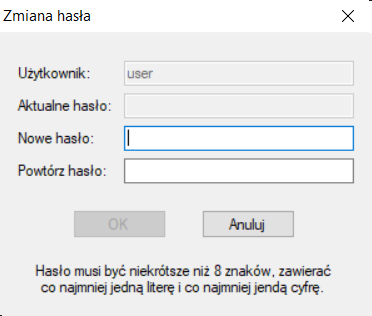
\includegraphics{obrazki/Logowanie/zmiana_hasla_uzytkownika.png}
	\caption{Okno zmiany hasła użytkownika}
	\label{zmianaHaslaUzytkownika}
\end{figure}
